\section{Basic principals}
When a discrete sequence $x[n]$ is applied to a system that gives the output $y[n]$ it is the impulse response of the system $h[n]$ that determined how the input sequence is affected. The output is determined by the convolution of input signal and impulse response of the system. \trine{include "LTI"}
\begin{align}
x[n]*h[n]=y[n]
\end{align}  
Such system is refereed to as a digital filter with impulse response $h[n]$ only letting selective frequencies through.\\ The frequency response of the filter is given by the Fourier transform of the impulse response, considering the input sequence $x[n]=e^{j\omega n}$ for $-\infty < n <\infty$, the frequency response is defined as\trine{side (40) DTSP}
\begin{align}
H(e^{j\omega})=\sum_{k=-\infty}^{\infty}h[k]e^{-j\omega k}
\end{align}
Hence the outcome of the filter becomes 
\begin{align}
y[n]=H(e^{j\omega})e^{-j\omega n} \label{eq:filter_output}
\end{align} 
By \eqref{eq:filter_output} it is seen that $H(e^{j\omega})$ describes the change in complex amplitude of a complex exponential input signal to a given frequency. $H(e^{j\omega})$ is in general complex and hence it can be expressed as
\begin{align}
H(e^{j\omega})=|H(e^{j\omega})|e^{j\measuredangle H(e^{j\omega})}
\end{align}  
where $|H(e^{j\omega})|$ and $e^{j\measuredangle H(e^{j\omega})}$ are functions of magnitude and phase response of the filter respectively, both real valued and $2\pi$-periodic.\\ If the frequency response of a filter is real it is said to have \textit{zero phase}, which is equavivalen to the phase response only tacking values that are integer multiples of $\pi$. Further if the frequency response can be written in the form 
\begin{align}
H(e^{j\omega})=A(e^{j\omega})e^{j(-\alpha\omega + j\beta)} 
\end{align}
where $\alpha$ and $\beta$ are constants and $A(e^{j\omega})$ is real,
the filter is said to have \textit{general linear phase}. That is because the phase response consist of constant terms added to the linear function making a straight line with slope $\alpha$ except from the discontinuities resolving from \\
\\

When designing filters it is ideal to have approximately constant magnitude and zero phase corresponding to the frequency response. Though for causal systems\trine{define} zero phase is not possible to obtain, hence some phase distortion is acceptable   

\section{Ideal filter} 

\begin{figure}[H]
\centering
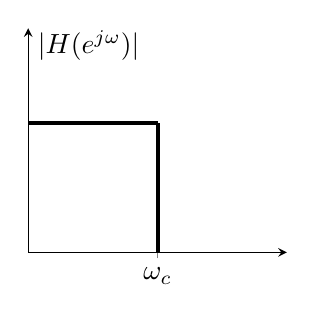
\begin{tikzpicture}[scale=1]
\begin{axis}[
scale=0.5,
unit vector ratio*=1 1 1,
axis lines = middle,
xtick={1.5},
xticklabels={$\omega_c$},
ytick=\empty,
xmin=0,
xmax=3,
ymin=0,
ymax=2.6]
\node at (axis cs:0.7,2.4) {$|H(e^{j\omega})|$};
\draw[line width=0.5mm](axis cs:0,1.5)--(axis cs:1.5,1.5);
\draw[line width=0.5mm](axis cs:1.5,1.5)--(axis cs:1.5,0);
\end{axis}
\end{tikzpicture}
\caption{}
\label{fig:lowpass}
\end{figure}

